% !TeX spellcheck = en_US
\documentclass[pdftex,english,oribibl]{llncs}

%% Spracheinstellungen laden
\usepackage[english]{babel}

%% Schriftart in der Ausgabe/Eingabe
\usepackage[T1]{fontenc}
\usepackage{textcomp}
\usepackage[utf8]{inputenc}

%% Zitate
\usepackage[numbers,sort]{natbib}
\bibliographystyle{abbrvnat}
%\bibliographystyle{dinat}
%\bibliographystyle{plainnat}
%\bibliographystyle{splncs}
%% Similar to option "sectionbib" but \refname instead of \bibname
\makeatletter
\renewcommand\bibsection{\section*{\refname\@mkboth{\MakeUppercase{\refname}}{\MakeUppercase{\refname}}}}
\makeatother

%% Index
%\usepackage{makeidx}
%\makeindex

%% PDF Einstellungen
% muss nach natbib geladen werden!
\usepackage{nameref}
\usepackage{varioref}
\usepackage[pdfusetitle,pdftex,colorlinks]{hyperref}
\hypersetup{pdfborder={0 0 0}}
\hypersetup{bookmarksdepth=3}
\hypersetup{bookmarksopen=true}
\hypersetup{bookmarksopenlevel=1}
\hypersetup{bookmarksnumbered=true}
\usepackage{color}
\hypersetup{colorlinks=false}

%\usepackage[section]{tocbibind}

\makeatletter
\gdef\@keywords{}
\def\keywords#1{\gdef\@keywords{#1}}
\gdef\@subtitle{}
\def\subtitle#1{\gdef\@subtitle{#1}}

%% modified from llncs
\renewenvironment{abstract}{%
  \list{}{\advance\topsep by0.35cm\relax\small%
          \leftmargin=1cm%
          \labelwidth=\z@%
          \listparindent=\z@%
          \itemindent\listparindent%
          \rightmargin\leftmargin}%
          \item[\hskip\labelsep\bfseries\abstractname]}{%
  \if!\@keywords!\else{\item[~]\item[\hskip\labelsep\bfseries\keywordname]\@keywords}\fi%
  \endlist}

\AtBeginDocument{%
  \if!\@subtitle!\else\hypersetup{pdfsubject={\@subtitle}}\fi
  \if!\@keywords!\else\hypersetup{pdfkeywords={\@keywords}}\fi
}
\makeatother

% llncs hyperref fix
\makeatletter
\providecommand*{\toclevel@author}{0}
\providecommand*{\toclevel@title}{0}
\makeatother

%% Mathe
\usepackage{amsmath}
\usepackage{amssymb}
\allowdisplaybreaks

%% Grafiken
\usepackage[pdftex]{graphicx}
\DeclareGraphicsExtensions{.pdf,.jpg,.png}


%% Listings
\usepackage{listings}
\lstset{escapechar=\%, frame=tb, basicstyle=\footnotesize}

%% Sonstiges
\newcommand{\TODO}[1]{\par\textcolor{red}{#1}\marginpar{\textcolor{red}{TODO}}}
\newcommand{\TODOX}[1]{\textcolor{red}{#1}\marginpar{\textcolor{red}{TODO}}}
\newcommand{\inlineQuote}[1]{``#1''}
\pagestyle{plain}

% Keine "Schusterjungen"
\clubpenalty = 10000
% Keine "Hurenkinder"
\widowpenalty = 10000 \displaywidowpenalty = 10000

%svg and pdf imports
\usepackage{svg}
\usepackage{pdfpages}

%
\usepackage{enumitem}
\def\labelitemi{$\circ$}
\usepackage{blindtext}
\usepackage{wrapfig}
\usepackage{placeins}

\usepackage[capitalise,nameinlink]{cleveref}

%tables
\usepackage{tabularx}
\usepackage{booktabs}
\usepackage{multicol}
\usepackage{makecell}


%figure and table caption setup
\usepackage{caption}
\captionsetup{labelfont=bf,format = hang,justification=raggedright }
\captionsetup[subfigure]{format = hang, labelfont=bf, position=b}
\usepackage{subcaption}
\usepackage{tikz}


%remove mathcal from Pi and Delta
\let\oldPi\Pi
\renewcommand{\Pi}{\ensuremath{\mathrm{\oldPi}}}
\let\oldDelta\Delta
\renewcommand{\Delta}{\ensuremath{\mathrm{\oldDelta}}}

%add normal braces to \ref command
\let\oldRef\ref
\renewcommand{\ref}[1]{(\oldRef{#1})}


%%%%%%%%%%%%%%%%%%%%%%%%%%%%%%%%%%%%%%%%%%%%%%%%%%%%%%%%%%%%%%%%%%%%%%%%%%%%%%%
%%% BEGIN DOCUMENT
%%%%%%%%%%%%%%%%%%%%%%%%%%%%%%%%%%%%%%%%%%%%%%%%%%%%%%%%%%%%%%%%%%%%%%%%%%%%%%%
\title{Learning and Predicting the Performance of Configurable Software Systems}
\subtitle{Seminar - Advanced Software Engineering:\\
Non-Functional Aspects in Software Engineering}
\author{Lion Wagner}
\institute{University of Stuttgart\\Institute of Software Technology (ISTE)\\70569 Stuttgart, Germany}

\newcommand\AFID{\hyperref[sec:AFID]{\textit{AFID}}}
\newcommand\VAPP{\hyperref[sec:VAPP]{\textit{VAPP}}}
\newcommand\WHAT{\hyperref[sec:WHAT]{\textbf{WHAT}}}
\newcommand{\CART}{\hyperref[sec:CART]{\textbf{CART}}}


\def\X{\ensuremath{\mathbf{X}}}
\def\Y{\ensuremath{\mathrm{Y}}}
\def\x{\ensuremath{\mathrm{\mathbf{x}}}}
\def\y{\ensuremath{\mathrm{y}}}



\setlength\intextsep{\baselineskip}
\begin{document}


\maketitle
\begin{abstract}
  Today's programs are mostly highly configurable and customizable. Popular applications like Apache or MySQL can have hundreds of configurable parameters. Whilst providing flexibility to a customer, this also brings some problems: having so many options can heavily influence the performance of a software system. And the more options there are, the harder it gets to predict the behavior of a software system. This paper will show that a brute force approach to this problem does not work as a general solution. Further it is going to explain and compare four different prediction methods that were developed by N. Siegmund et al. The comparison of those methods shows, that there is no 'best' approach to this problem, but rather a broad selection of well working methods exists. 
\end{abstract}


\section{Introduction} \label{sec:introduction}
Todays programs are mostly highly configurable and customizable. Popular applications like Apache or MySQL can have a lot of configuration parameters as can be seen in \cref{fig:paramters}. With this large amount of  configuration options stake holders or customers can be satisfied easier since they can tailor a program to the their specific requirements. But with these big amount of options comes a bigger problem: \inlineQuote{unpredictability}. Looking at an example of Apache Storm (\cref{fig:ApacheStorm}) shows that the performance of two configurations of a program can differ significantly. \TODOX{figure einfügen} shows that solely changing a single parameter can increase the response time of Apache Storm by up to 100\%. Without using prediction methods such results are only visible after executing and measuring multiple, if not all, configurations of a system. Or in other words: when looking only at a single configuration, one cannot conclude whether that configuration is any good for the current requirements in.

\begin{figure}[h]
	\centering
	\includegraphics[clip,trim= 11cm 13cm 2cm 7cm]{Paper/thirdParty/HeyYouHaveGivenMeTooManyKnobs.pdf}
	\caption{Number of parameters of different popular programs \cite{YouveGivenMeTooManyKnobs}.}
	\label{fig:paramters}
\end{figure}\noindent
\begin{figure}[h]\noindent
	\begin{subfigure}{.45\linewidth}
		\centering
		\includegraphics[page=5,clip,trim=4cm 1cm 8cm 10cm,width=\linewidth]
		{Paper/thirdParty/vamos_keynote_norbert_siegmund.pdf}
		\caption{Configurations of Apache Storm sorted by measured throughput.}
	\end{subfigure}\hspace{.1\linewidth}
	\begin{subfigure}{.45\linewidth}
		\centering
		\includegraphics[page=5,clip,trim=17.4cm 1cm 0cm 10cm,width=.8\linewidth]
		{Paper/thirdParty/vamos_keynote_norbert_siegmund.pdf}
		\caption{Possible influences of only two options on the latency of Apache Storm. }
	\end{subfigure}
	\caption{Measurements done for Apache Strom that show an configurations can have a significant influence on the performance of a software system.}
	\label{fig:ApacheStorm}
\end{figure}


This is where prediction comes into play. By learning about the performance of some configurations of the system it tries to generates a function that can give an expected performance for a not measured configuration. This can be used to solve the just mention problem of finding a near optimal solution.
Further performance prediction can be used to find default configurations. These should be configurations that fulfills most requirements to an acceptable level. 
The most straight forward  approach to this problem would be a \textit{brute-force} solution. In this case that would mean measuring each and every single valid configuration. As we will see later in \TODOX{ref section} this approach is in general not feasible since the amount of valid configurations scales exponentially with the number of parameters. For that reason other approaches had to be found and especially the efficient sampling of a configuration space turned out to be a problem \cite{CostEfficientSampling_Gou_Siegmund_2015}. 

This paper will focus on showing different approaches and strategies to predicting the performance of a configurable software system. It will mainly discuss approaches developed by Norbert Siegmund et al. \cite{AutomatedFeatureDetectionSiegmund2012,VariabilityAwarePerformancePredictionJianmeiSigmundApel,CostEfficientSampling_Gou_Siegmund_2015, DistanceBasedSampling2019}. They will be explained and compared. More specificly this paper will have a look at 4 different approaches besides \textit{brute-force}.

The first discussed technique is \textit{Automated Feature Interaction Detection} (\AFID) \cite{AutomatedFeatureDetectionSiegmund2012}. The goal of this approach is to assign a performance influence value to each feature and feature interaction. This is done by observing and measuring the behavior of certain configurations. 
The other 4 approaches make use of a CART Tree as their learning choice but differ in the way they choose their sample. 
\textit{Variability Aware Performance Prediction} (\VAPP) \cite{VariabilityAwarePerformancePredictionJianmeiSigmundApel} uses random sampling to pick which configurations to compiled and measured. 
\WHAT~ \cite{DistanceBasedSampling2019}, as the next approach is called, tires a more mathematical way to find groups of similar configurations without actually measuring them. For this distance based clustering/sampling is used. 
The last two sampling approaches are proposed in the same paper by \citet{CostEfficientSampling_Gou_Siegmund_2015}. They \textit{Progressive} and \textit{Projective Sampling} are quite similar, since they both take advantage of the fact, that the general formular behind a learning curve is known. With this knowledge they generate a part of the actual curve and fit a function to it. Based on this function a optimal size for the actual sample set can be calculated. Both methods also take the cost of measurements and over-/underfitting into consideration.\\
All these approaches reach an accuracy of over 94\% on average in the conducted tests of their corresponding papers. This makes them good enough to be relevant for the topic of this paper.

\section{Definitions}

Before the actual approaches are discussed it is important to pin point the definitions of terms which are used in this paper.

This paper often uses the terms \inlineQuote{parameters}, (configuration-)\inlineQuote{options} or \inlineQuote{features}. These terms are all equivalent and describe ways to adjust and optimize functional and non-functional properties of a software system \cite{DistanceBasedSampling2019}.
One can divide into different types of options. Binary options usually have a value of 0 or 1 and describe the activation of a feature. Non-binary options support a wider range of values. For example this could be a setting for the stack-size allowed for a program. Non-Numeric options support the input of text. Those could be paths or other addresses.
The set of all configuration options is denoted as $\mathcal{O}$.


A \textit{configuration} can be defined in multiple different ways. \citet{DistanceBasedSampling2019} define a configuration as a function $c : \mathcal{O} \rightarrow \{0,1\}$. It assigns a 1 to each element of $\mathcal{O}$ that is selected and a 0 to those which are not used.
\citet{FasterDiscoveryofFasterSystemConfigurationsSiegmund2017} and \cite{VariabilityAwarePerformancePredictionJianmeiSigmundApel} have a similar approach. But instead of using a function to describe $c$ they use a vector or a n-tupel over $\mathbb{Z}^+_2(= \{0,1\})$. Each position of those enumerations is associated with exactly one feature. As in \cite{DistanceBasedSampling2019} a 1 indicates an activation of a feature and a 0 means that the feature is not used. These definitions obviously describes binary options only, but can be expanded to support non-binary options by using the codomain of $\mathbb{N}_0$ instead of $\{0,1\}$.

The \textit{configuration space} describes all valid configurations of a system. It is denoted as $\mathcal{C}$.

A \textit{sample} is the subset of a \textit{configuration space} that contains all configurations that are complied and measured during the process of sampling and learning.



\section{On the Applicability of the Brute Force Approach}
\label{sec:BruteForce}
As mentioned previously: \textit{brute force} measuring is not feasible in most cases \cite{AutomatedFeatureDetectionSiegmund2012}. But what is the actual reason behind this?
Let's have a look at an example first:

In one paper, \citet{AutomatedFeatureDetectionSiegmund2012} measured all valid configurations of multiple programs to analyse the accuracy of \AFID. Berkley DB (C) was one of those programs. It is a database management program for embedded systems. It has 19 features and 2560 valid configuration. In the end, it took approximately 426 hours (= 17.75 days) to measure all these configurations. This value calculates to a time of about 10 minutes per configuration measurement. Considering that Berkeley DB (C) is a comparably small program, this is already a significant amount of time but still a time span that might be acceptable be used to get the perfect results of a \textit{brute force} approach.

This changes once one takes a look at larger programs. Modern applications like Apache or MySQL can have hundreds of configuration parameters \cite{YouveGivenMeTooManyKnobs}. Another example was displayed by \citet{VAMOSConference}: SQLite has 77 features that can produce $3 \cdot 10^{77}$ valid configurations. Unfortunately, there is no evidence how the latter number was calculated. Yet, it can be assumed that at least the scale of this number in regard to the number of features is correct. This will be explained in the next paragraph. Coming back to the example: Assuming measuring (compiling + profiling) one configuration would take 5 minutes, a brute-force approach would take $2.5 \cdot 10^{76}$ hours. Obviously, this is not an acceptable duration.

\begin{wrapfigure}{r}{0.5\textwidth}
	\includegraphics[width = 0.5\textwidth]{presentation/figures/FeatureModel}
	\captionsetup{width=0.95\linewidth}
	\caption{An example of a feature model.}
	\label{fig:FeatureModel}
\end{wrapfigure}

To find out why \textit{brute-force} does not scale well, a generic look at how many configurations per program are needed to be measured helps. This set of all valid configurations can be written down as a \textit{Feature Model}. An example for this is shown in \cref{fig:FeatureModel}. This \textit{feature model} describes the software system called \inlineQuote{DatabaseSystem}. \textit{Feature Models} can be annotated with further logical expressions to also contain cross-feature constraints. Such can also be seen in the just mentioned example. Each \textit{Feature Model} can also be written down as a logical expression. The atomic variables of this expression are the options of the software system. In this context, a configuration is written down as an assignment of each variable of the expression. The tree in \cref{fig:FeatureModel} is equivalent to the function
\begin{equation*}
	V(C)= \text{Base} \land (\text{Version1.5} \oplus \text{Version2.1}) \land (\text{Version1.5} \Rightarrow \neg \text{DBServer}).%Punkt gehört zum Satz
\end{equation*}
For $V(C)=1$, a configuration is considered \textit{valid}. Otherwise, it is not accepted.
An example configuration could look like this:
\begin{align*}
	\textbf{DEFAULT} =  \{&\text{Base} = 1, \text{Version1.5}=0, \text{Version2.1} = 1, \\
	&\text{DBServer} =0, \text{SearchEngine} =0 \}
\end{align*}
Note that these logical expressions can also be applied to non-binary options. The feature \inlineQuote{Base} of the example could also be expressed as a tertiary value:

\begin{equation*}
	\text{Base} =  \begin{cases}
		0, \text{Not selected}\\
		1, \text{Version1.5 selected}\\
		2, \text{Version2.1 selected}
	\end{cases}
\end{equation*}
$V(C)$ would look like this, if Base is tertiary:
\begin{equation*}
		V(C)= (\text{Base} \Leftrightarrow 1 \lor \text{Base} \Leftrightarrow 2) \land \big((\text{Base} \Leftrightarrow 1) \Rightarrow \neg \text{DBServer}\big).
\end{equation*}
\noindent
In this context the most interesting property of this formula is the scaling of the number of valid configurations in relation to the number of options. Without loss of generality, one can assume that a system only has binary options. This can be done since all other types of options would just increase the overall number of options. However, already looking at binary options gives a satisfying result. Since naturally the total number of possible assignments for a logical expression is exponentially large, the number of valid configurations also lies in the exponential space of $\mathcal{O}(2^{\#options})$. In other words: a \textit{configuration space} that would have to measured for a \textit{brute force} approach would be exponentially large. 
This exponential scaling is also the reason why brute-force does not scale well and more sophisticated methods are need for efficient predictions.




%\section{Software Product Lines}

As mentioned in the \hyperref[sec:introduction]{introduction} modern software systems are often highly configurable and customizable. To be able to provide such a large amount of customization, software engineers adopted the concept of \textit{mass customization}. A technique mostly known from the automotive industry \cite{SPLEngineering}. It involves the building of a product line that supports the output of highly customizable products. The result of bringing \textit{mass customization} into software development are Software Product Lines (SPL). SPLs are broadly found throughout software development and in all kinds of development environments \cite{Reportof2010USArmySPLWorkshop,DynamicSoftwareProductLines}. 

\subsection{Introduction into Software Product Lines}\label{sec:SPLIntroduction}
\citet{SPLEngineering} describe how a general product-line functions: There is a \textit{common platform}, which is in itself expandable and holds all basic functionalities. It also provides interfaces for adding on parts (features). Some parts are mandatory and some are optional. For each part there might be different versions or variations that are interchangeable.\\
Applying the factor software engineering to this general product line leads one to the definition of SPLs by the Software Engineering Institute (SEI, \url{https://www.sei.cmu.edu/}): \inlineQuote{[...] a set	of software-intensive systems that share a common, managed set	of features satisfying the specific	needs of a particular market segment or mission and that are developed from a common set of core assets in a prescribed way.}\cite{SalionIncASPLCaseStudy}.


\begin{figure}
	\centering
	\setlength\belowcaptionskip{-\baselineskip}
	\captionsetup{width=0.95\linewidth}
	\includesvg[scale = 0.7]{figures/VisualStudioSPL.svg}
	\caption{Partial view of the Visual Studio Product Line \cite{VisualStudioSPL}. (Assuming a Microsoft is using core libaries for its product. Which is likely since .Net Core runs on all major operating systems.) }
	\label{fig:VSSPL}
\end{figure}\noindent
In particular SPLs inherit the behavior of reusing existing components to enhance the development process \cite{IssuesAndModelsInSPL}. A more detailed look at the economical thought behind SPLs is given by \citet{IssuesAndModelsInSPL}.\\
An example of a SPL would be the Visual Studio product line from Microsoft as shown in \autoref{fig:VSSPL}. The common platform are some core libraries that provide shared code to all products of this line. The products themselves add platform or usage specific features (parts) to the core to offer a broad variation of products. The Visual Studio IDE even splits up further into 3 products that all serve a different purpose, but use same code base. Note that \hyperref[fig:VSSPL]{figure 1} only displays static variations of the product line. Almost all versions are additionally dynamically expendable via plug-ins and customizable via options and preferences.

\subsection{Performance Influences of Feature Binding in SPLs}\label{sec:SPLPerformanceInfluence}

The following section is based on Combining Static and Dynamic Feature Binding in Software Product Lines~by~\citet{CombiningStaticandDynamicFeatureBinding}.\\
This paper will use the terms \textit{feature} and \textit{configuration} as they are defined in \cite{AutomatedFeatureDetectionSiegmund2012} \inlineQuote{[...], where a feature is a stakeholder-visible behavior or characteristic of a program.} and a \inlineQuote{a specific set of features, [is] called a configuration}.\\
When designing a SPL one has a choice for each feature to either bind it statically or dynamically.
A statically bound feature is compiled directly into the binary of a program. Its always available to the environment when needed but uses up binary space to do so.
When dynamically binding a feature it is not a part of the core binary, yet a part of an external \textit{feature library}. Once such a feature is needed the core loads the according library from an external source. This leads to the core binary being smaller but the size needed for each feature is increased by some meta-data (size, location, format, etc. of the feature library). Multiple features can be combined into one feature library for optimization. Feature libraries are also called \textit{binding units}. Note that \cite{CombiningStaticandDynamicFeatureBinding} uses the \textit{decorator pattern} for the realization of dynamic feature binding.\\
To describe the effects of binding types we use the terms \textit{functional} and \textit{compositional overhead}. A functional overhead  originates form features (or binding units) that are loaded inside a program yet never used. In turn a compositional overhead is found as meta data that is needed to describe dynamic behavior.\\An abstract example: A program core consisting out of 3 features and uses up~2MB of (hard-drive) memory. We extract 1 feature that is rarely used into a dynamic link library with the size of~1.1MB. Afterwards our core is only~1MB large. We can already conclude that our original program had a functional overhead of~1MB by subtracting the old and the new binary size. When using the extracted feature our program uses up~2.1MB of memory. So we can say that our compositional overhead for extracting the feature is 0.1MB. That is the data needed to describe the location, format, etc. of the feature library.\\
\TODO{daten aus paper einfügen}
\TODO{Fig 18 einbauen}
Coming back to binding types we have the problem of finding an optimal combination of static and dynamic bindings. \citet{CombiningStaticandDynamicFeatureBinding} suggest to prefer static binding if no dynamic extensibility is required and resources are not limited. A full static bound program has no compositional overhead and thus only requires additional (persistent and transient) memory. However programs that are more limited in their resources may need to be designed to minimize the overall overhead. This is basically the same task of finding an optimal configuration of a program. Techniques regarding the analysis and prediction will come up later in \cref{sec:measuring}. The compositional overhead of binding units can be predicted partially since feature libaries have a constant size header (e.g. 5KB per Dynamic Link Library \{DLL\}). A general guideline is to avoid a large number and a large size of binding units. Overlapping binding units as well as dynamic splitting and merging of binding units are possible optimizations. \citet{CombiningStaticandDynamicFeatureBinding} also mention that \inlineQuote{[...] there is no optimal size for a binding unit, a domain expert can define binding units per application scenario.}.
\section{Measuring and Predicting the Performance of Highly Configurable Systems}

As already established modern programs have a lot of customization options.
With such a large amount of configuration options a developer needs some sort of mechanism to ensure his application has the required performance under most or all configurations. On one hand this is very important when it comes to contract terms and conditions with customers. A program should perform as good as the customer needs it to. Otherwise a developer may face fines. On the other hand performance prediction is helpful in finding performance problems or room for improvement. This either helps with the previous point of reaching a set performance target or to make the program more user friendly (less response time, smaller binary size, ...).\\
It is important to note that since we have such a large configuration space one can only talk about the average performance of either a program (considering all configurations) or the performance of a specific configuration(-family)/feature.\\
Why do we need to learn and predict the performance of a system? Berkley DB (C) is a database management program for embedded systems. It has 18 features and 2560 different configurations. In their paper \inlineQuote{{\textit{Predicting Performance via Automated Feature-Interaction Detection}}} \citet{AutomatedFeatureDetectionSiegmund2012} measured each configuration and it took 426h (=17,75d)\footnote{These measurements were done on computers that are (from today's point of view) fairly slow \cite{AutomatedFeatureDetectionSiegmund2012,CPUDatabase}. }. This and other examples from the same paper show, that it is not practical to brute force measure each and every configuration possible.\\
By learning about the performance difference between multiple configurations it is possible accurately predict the behaviour of a program. This means that one does not need ot measure all possible configurations but instead a small sample size should be enought to predict a programs performance. This can be done in multiple ways. This paper will take a look at \hyperref[sec:AFID]{Automated Feature Interaction Detection}, a statistic based approach and WHAT (machine/spectral learning).

%\subsection{On the Problem of Measuring a Configurable Software System}


\subsection{Automated Feature Interaction Detection}\label{sec:AFID}

Automated feature interaction detection (\AFID) is a measurement-based approach to predicting the performance of a highly configurable system.
It was developed by \citet{AutomatedFeatureDetectionSiegmund2012}. The following section is also based on the proposing paper of \AFID~\cite{AutomatedFeatureDetectionSiegmund2012}. 

Under the usage of linear regression \AFID~tries to determine a performance influence value for each feature and feature interactions. A feature interaction is defined as a unexpected influence on the performance of a system when using a specific feature combination.
In the conducted experiments of \citet{AutomatedFeatureDetectionSiegmund2012} and \citet{CostEfficientSampling_Gou_Siegmund_2015} this method reaches average accuracies of  respectively 95\% and 85\%.
\\
\noindent
In general one can divide \AFID~into two different steps:
\begin{enumerate}
	\item Find interacting Features.
	\item Measure the performance influence of feature interactions.
\end{enumerate}
Firstly step some notation is needed. For simplicity \AFID~is defined for binary options.
\TODOX{Add overview graphic}
The composition of performance influencing units (features or feature interactions) is denoted by a $\cdot$. If two features are used simultaneously it is denoted by using a $\times$. This would also be another way to describe a configuration. So a program $P$ that uses the two features $a$ and $b$ can be denoted as $P= a \times b$.\\
If one now wants to know the performance of $P$, they have to calculate $\Pi(P)$. The exact definition of the performance influence determining function $\Pi$ can be found in the paper of \citet{AutomatedFeatureDetectionSiegmund2012}. For now it is important to note that when calculating $\Pi(P)=\Pi(a \times b)$ not only the performance influence of $a$ and $b$ are necessary but also has $a\#b$ has to be considered. The latter is the performance influence of the possible interaction between $a$ and $b$. So $\Pi(a \times b) = \Pi(a\#b) + \Pi(a) + \Pi(b)$. This can also go into higher order interaction: When using a program configuration $P_2 = a \times b \times c$ then $\Pi(P_2) = \Pi(a) +  \Pi(b) +  \Pi(c) +  \Pi(a\#b) +  \Pi(a\#c) +  \Pi(b\#c) +  \Pi(a\#b\#c)$. Some interactions do not exist or have an influence on the system, those who actually have have to be found and measured. Otherwise one could end up doing a brute-force solution again.\\\\

Finding these interactions requires to find the related interacting features themselves first.
This is done in by intelligently measuring certain configurations. \AFID~defines a features $a$ as interacting when
\begin{equation}\label{def:equation}
a \text{ interacts} \Leftrightarrow \exists C,D \subseteq \mathcal{C}| C \neq D  \land	 |\Delta a_C - \Delta a_D| \leq t
\end{equation}
with 
\begin{equation}
\begin{split}
\Delta a_C &= \Pi(C\times a) - \Pi(C)\\
&=\Pi(a\# C) + \Pi(a).
\end{split}
\end{equation}
$t$ is a threshold depending on the given performance metric.
Using these two equations one can determine whether a feature is interacting with other features using 4 measurements.
These include $\Delta a_{min} = \Pi(a \times min(a)) - \Pi(min(a))$ and $\Delta a_{max} = \Pi(a \times max(a)) - \Pi(max(a))$. $min(a)$ is a configuration that contains the minimum possible features without using $a$. Simultaneously $max(a)$ is also a configuration that contains the maximum amount of possible features without $a$. 
Once these measurements are done \cref{def:equation} can be applied with $C=\Delta a_{min}$ and $D=\Delta a_{max}$. This is done for all features to find interacting ones.
If a feature $f$ is not found to be interactive its performance influence  $\Pi(f)$ equals $\Delta f_{min}$.


Once all interacting features are found the search for the actual interactions starts. In this second step 3 different heuristics are used to determine which interactions are searched for.
 
 \newcommand{\oitem}[2]{{\item[{\parbox[t][0pt][t]{\leftmargin}{\raggedleft #1}}] {\parbox[t]{\textwidth-\leftmargin}{#2}}}}
 \begin{itemize}[leftmargin=4cm]
 	\setlength\itemsep{1em}
 	\oitem{Pair-Wise~Heuristik (PW):\label{lab:PW}}{ Most groups of interacting features appear in the size of two \cite{AutomatedFeatureDetectionSiegmund2012,AnalysisOfTheVariabilityInFortyPreprocessor_BasedSPLLiebig}. So it makes sense to look for pair interaction first.}
 	\oitem{Higher-Order Interactions Heuristic (HO):\label{lab:HO}}{
 		\citet{AutomatedFeatureDetectionSiegmund2012} only look at higher order interactions of the rank of three. Even ranks would take up to much measurement resources.
 	}
 	\oitem{Hot-Spot Features (HS):\label{lab:HS}}{
 		Based on \cite{FeatureCohesioninSPL, CanWeAvoidHighCoupling?} \citet{AutomatedFeatureDetectionSiegmund2012} assume that hot spot features exist. At last these specific type of interactions are findable too.
 	}
 \end{itemize}
Using a SAT-Solver an implication graph as seen in \autoref{fig:ImplicationTree} is generated. Each implication chain in this tree should have at least one interacting feature. When analysing the tree each chain is walked from the top down. The three heuristics will be applied in the order of PW $\rightarrow$ HO $\rightarrow$HS.  

\begin{wrapfigure}{l}{0.5\textwidth}
%\setlength\belowcaptionskip{-\baselineskip}
\includesvg[width = 0.5\textwidth]{figures/ImplicationTree}
\captionsetup{width=0.95\linewidth}
\caption{Implication tree example found in \cite{AutomatedFeatureDetectionSiegmund2012} }
\label{fig:ImplicationTree}
\end{wrapfigure}

First the influence of every feature on another chain is measured (\hyperref[lab:PW]{PW-heuristic}). In the example of \autoref{fig:ImplicationTree} the interactions would be measured in this order:\inlineQuote{$F1\#F6, F1\#F7, F4\#F6,\\ F4\#F7, F6\#F11,F7\#F11,F1\#F11,\\ F4\#F11$}\cite{AutomatedFeatureDetectionSiegmund2012}. If an interaction impact $\Delta a\#b_C$ exceeds a threshold it is recorded.

Secondly, the \hyperref[lab:HO]{higher order interaction heuristic} is applied. Higher order interactions can be relatively easily found by looking hat the results of the PW-Heuristik. Three features that interact pair-wise are likely to interact in a third order interaction. For example, looking at features $a$, $b$ and $c$- If $\Delta a\#b_{C1}$ and $\Delta b\#c_{C2}$ have been recorded $\{a\#b, b\#c, a\#c\}$ all have to be non zero to find a third order interaction. Interactions with and order higher than three are not considered to prevent too many measurements.

Lastly Hot-Spot features are detected (\hyperref[lab:HS]{HS-heuristic}). This is done by counting the interactions per feature. If the number of interactions of a feature is above a certain threshold (e.g. the arithmetic mean) it is categorized as a Hot-Spot feature. Based on the hotspot features further third order interactions are explored. Again higher order interactions are not considered to prevent too many measurements. \\
After applying the three heuristics all detected interacting features or feature combinations are assigned a $\Delta$ to represent their performance influence on the program.

\begin{wrapfigure}{r}{.5\textwidth}
	\centering
	\setlength\belowcaptionskip{-2\baselineskip}
	\captionof{table}{Results of average accurcy found by \citet{AutomatedFeatureDetectionSiegmund2012}}
	\label{tab:avgAccuracy}
	\begin{tabular}{c|c}
		Approach&avg. Accuracy\\\midrule[1pt]
		FW&79.7\%\\\hline
		PW&91\%\\\hline
		HO&93.7\%\\\hline
		HS&95.4\%\\\hline
	\end{tabular}
\end{wrapfigure}\noindent
\citet{AutomatedFeatureDetectionSiegmund2012} tested AFID on six different SPLs (Berkely DB C,Berkely DB Java, Apache, SQLite, LLVM, x264). Each program was tested under four approaches: Feature-Wise, Pair-Wise, Higher-Order, Hot-Spot (in this order). Each approach also used the data found by the previous one. Accordingly the results get better the more heuristics are used as seen in \cref{tab:avgAccuracy}. Using only the FW approach means that interactions (and the heuristics) are not considered, yet the accuracy is already at about 80\% on average. A significant improvement can be made by using the PW heuristic. It uses on average 8.5 times more measurements than the FW approach but improves the accuracy to 91\%. Using the HO or HS approach improves the accuracy further by about 2-4\%. However for Apache using the HO over the PW approach even deteriorated the average result by 3.9\% and doubled the standard variation. As already mentioned using the HS approach gives the best accuracy this is true for all 6 tested applications. \citet{AutomatedFeatureDetectionSiegmund2012} also notes that analysing SQLite only needed about 0.1\% of all possible configurations. This hints to the good scalability of AFID.

\subsection{Variability aware Performance Prediction}\label{sec:VAPP}

The following section is based upon \citet{VariabilityAwarePerformancePredictionJianmeiSigmundApel}.\\
Variability aware Performance Prediction (\VAPP) is a statistics based approach to performance prediction. With the help of random sampling and \CART s a simple yet effective predictor can be build. In their own tests \citet{VariabilityAwarePerformancePredictionJianmeiSigmundApel} reached an average precision of 94\% whilst using a sample as large as the ones \AFID would be using under the PW heuristic. Further tests conducted by \citet{FasterDiscoveryofFasterSystemConfigurationsSiegmund2017} with the same sample size showed an accuracy of 92.4\%. 


\begin{wrapfigure}{r}{.5\linewidth}
	\vspace{-1\baselineskip}
	\setlength\belowcaptionskip{-\baselineskip}
	\includegraphics[page=3,clip,trim=11cm 13.5cm 1.5cm 10.25cm, width=\linewidth ]{Paper/VariabilityAwarePerformancePredictionAStatisticalLearningApproach}
	\caption{Overview of the Approach of Variability aware Performance Prediction \cite{VariabilityAwarePerformancePredictionJianmeiSigmundApel}}.
	\label{fig:VAPPOverview}
\end{wrapfigure}

\subsubsection[Basic Idea]{\textnormal{The} basic idea} of variability aware performance prediction can be seen in \autoref{fig:VAPPOverview}.

Two cycles can be found. 

The first cycle is outside of the dashed box and describes the basic input-output behaviour of a predictor. A user configures a new configuration $\x$ for System $A$ and asks the predictor (dashed box) for a prediction. It replies with a quantitative prediction for $\x$'s performance.

In the second cycle a actual prediction is generated based on decision rules which themselves are inturn created by simplifying a performance model (a \CART). Random sampling is used to learn the performance model.
\\\\
Like other approaches, the target of variability aware performance prediction is to get accurate predictions with only using a small sample for the creation of the performance model.

\FloatBarrier %forces the float to appear below the subsubsection
\subsubsection{Statistical Methods}\label{sec:VAPPMethods} are used to perform the actual computation. First of all a configuration is defined as an $N$-tuple $(x_1,x_2,x_3,...,x_N)$, where $N$ is the number of all available features. Each $x_i$ represents a feature and can either have the value 1 or 0 depending on whether the feature is selected or not. An actual configuration example would be $\x_j = (x_1=1,x_2=0,x_3=1,\dots,x_N = 1)$. All valid configurations of a system are denoted as $\X$.\\

\VAPP~uses the tupel definition of a configuration. It further defines that for each configuration of $\mathcal{C}$ an actual performance value $y_j$ can be assigned. $\Y$ denotes the performance of all configurations of a system.\\
For formal correctness it is assumed that each option of a configuration actually influences the performance of the system. Otherwise a \CART could not be applied.

Combining $\Y_\X$ with $\X_\mathcal{C}\subset\mathcal{C}$ gives a sample $S$. $\Y_\X$ are the to $\X_C$ associated and measured performance values. Now the two problems arise that \VAPP tries to solve:
\begin{enumerate}
	\item Predict the performance of the not measured configurations $\hat{=}\;\X\backslash\X_\mathcal{C}$.
	\item Find a function $f$ that shows the correlation between $\X_\mathcal{C}$ and $Y_\X$ and that makes each predicted performance $f(\x)$ of $\x$ as close as possible to its actual performance.\\	
	\begin{equation}
	f : \mathcal{C} \rightarrow  \mathbb{R} \text{ such that} \sum_{\x,y \in S} L(y,f(\x)) \text{ is minimal}
	\end{equation}\\
	 $L$ is a loss function to penalize errors in prediction.
\end{enumerate}
This is done with the help of CART. All sample configurations get categorized into a binary trees leafs. A configurations selection of features determines its location in the tree. The distribution of samples inside the tree is determined with the goal of minimizing the total prediction errors per segment (sub-trees). An example tree can be found in \cref{fig:VAPPExampleTree}.
For each leaf one can determine the \textit{local model} $\ell$
\begin{equation}
	\ell_{S_i} = \frac{1}{|S_i|} \sum_{y_j \in S_i} y_j
\end{equation}
As a loss function to penalize the prediction errors \citet{VariabilityAwarePerformancePredictionJianmeiSigmundApel} choose the sum of squared error loss:
\begin{equation}
	\sum_{y_j \in S_i} L(y_i,\ell_{S_i}) = \sum_{y_j \in S_i} (y_j - \ell_{S_i})^2
\end{equation}
Therefore the best split for a segment $S_i$ is found when
\begin{equation*}
\sum_{y_j \in S_{iL}} L(y_i,\ell_{S_{iL}}) + \sum_{y_j \in S_{iR}} L(y_i,\ell_{S_{iR}})
\end{equation*}
is minimal. To prevent \textit{under}- or \textit{overfitting}\cite{ElementsOfStatisticalLearning} the recursive splitting has to be stopped at the right time. This is possible by manual parameter tuning or using a empirical-determined automatic terminator. \\
Now to the actual calculation of the quantitative prediction. Assuming there are $q$ leafs in our tree than $f(\mathrm{x})$ is defined as:
\begin{equation}\textsl{}
f(\mathrm{x})=\sum_{i=1}^{q} \ell_{S_i}I(\mathrm{x}\in S_i)
\end{equation}
where $I(\mathrm{x}\in S_i)$ is an indicator function to indicates that $\mathrm{x}$ belongs to a leaf $S_i$.\\
For the example of \autoref{fig:VAPPExampleTree} $f(\mathrm{x})$ unwraps to:
\begin{align*}
f(x) = 255&* I(x_{14}=1,x_7=0)\\[-0.1cm]
	 + 268&* I(x_{14}=1,x_7=1)\\[-0.1cm]
	 + 402&* I(x_{14}=0,x_{15}=1,x_3=0)\\[-0.1cm]
	 + 508&* I(x_{14}=0,x_{15}=1,x_3=1)\\[-0.1cm]
	 + 571&* I(x_{14}=0,x_{15}=0,x_3=1)\\[-0.1cm]
	 + 626&* I(x_{14}=0,x_{15}=0,x_3=0)
\end{align*}
Every possible configuration $\mathrm{x}$ is associated with a leaf of the tree. Therefore $f(\mathrm{x})$ can always be applied.\\
For their Experiment \citet{VariabilityAwarePerformancePredictionJianmeiSigmundApel} test the same software systems as \citet{AutomatedFeatureDetectionSiegmund2012} (\cref{sec:AFID}). They also compare their prediction results with the results produced by SPLConquerer under \AFID.\\
Unlike \AFID~the size of a sample for variability aware performance prediction can be chosen freely. \citet{VariabilityAwarePerformancePredictionJianmeiSigmundApel} use 4 different sample sizes based on the size of the program. For a program with $N$ features they use samples the size of $N,2N,3N \text{ and } M$. $M$ is the amount of configurations measured by SPLConquerer's using the \hyperref[lab:PW]{PW heuristic}.
It is found that the prediction accuracy increases linear with the size of the sample. It is also found that for using a small sample with the size of $N$ the prediction accuracy was at 92\%. However for Berkeley DB (C) the prediction rate with $N$ sized samples was at 112.4$\pm$354.6\%\footnote{$\pm$354.6 indicates the standard deviation}. This results into an average accuracy of only 28.6$\pm$68.9\%. Using a sample size of $M$ significantly improves the average prediction accuracy to 93.8\%.\\
Further \citet{VariabilityAwarePerformancePredictionJianmeiSigmundApel} comparer their approach with \AFID. This can be done since $N$ also equals the amount of configurations measured by the \hyperref[lab:FW]{FW heuristic}.\\
As already established variability aware performance prediction is not accurate for small sample sizes so it is no surprise that \AFID~with the \hyperref[lab:FW]{FW heuristic} performace better at $20.3\pm21.2$\% with a sample size of $N$. However, when using samples of size $M$ SPLConquerer's \hyperref[lab:PW]{PW heuristic} only reaches an average precision of 90.9\% compared to the already mentioned 93.9\% of \citet{VariabilityAwarePerformancePredictionJianmeiSigmundApel}'s approach.
Using the \hyperref[lab:HO]{HO} or \hyperref[lab:HS]{HS heuristic} of \AFID can produce a precision of up to 95\% but requires more measurements. This is not covered by \cite{VariabilityAwarePerformancePredictionJianmeiSigmundApel}.
%TODO vllt selbst prüfen?

\subsection{WHAT}\label{sec:WHAT}


%The test also show that for a low number of features a Brute-Force (BF) approach might also be viable. Measuring all configurations of Apache took about 213h where as the HS approach took 159h. BF guarantees a 100\% correct prediction where as the HS approach only had 94.7\% accuracy. Its is also worth noting that these tests were done on computers that are (from today's point of view) fairly slow \cite{CPUDatabase}. 

%Performance problems occuring after a while are not covered or predictable by these solutions. They go back to the old Holding problem


% !TeX spellcheck = en_US
\section{Comparison}
\begin{figure}[t]
	\centering
	\captionof{table}{Measureing results of \citet{FasterDiscoveryofFasterSystemConfigurationsSiegmund2017} when comparing the methods of, \AFID(Siegmund), \VAPP(Gou), \WHAT~and projective sampling in combination with CARTs (Sarkar). The \textit{Rank} column is computed using Scott-Knott, bootstrap 95\% confidence, and A12 test \cite{FasterDiscoveryofFasterSystemConfigurationsSiegmund2017}.}
	\label{tab:ConclusionPerformanceOverview}
	\vspace{-.5\baselineskip}
	\includegraphics[page=19, clip=true, trim=2.5cm 13.8cm 6.8cm 3.1cm, width=.9\linewidth]{"Paper/Faster Discovery of Faster System Configurations with Spectral Learning".pdf}
	\vspace{-1\baselineskip}	
\end{figure}
\cref{tab:ConclusionPerformanceOverview} displays the results of an experiment conducted by \citet{FasterDiscoveryofFasterSystemConfigurationsSiegmund2017}, to compare the different prediction methods. The table shows some characteristic properties of each approach.

Siegmund's approach of \AFID~was ranked last on 4 occasions. Its accuracy and standard deviation are the worst in most cases. It mostly ranks lower than \VAPP~whilst utilizing same sample size (Guo(PW)). \WHAT~is the oldest of the presented approaches and its low ranking can be seen as a demonstration on how prediction algorithms evolved over time.

Both versions of \VAPP~appear inconsistently with regard to their rank. Gou(PW) ranks lower than Gou(2N) in half of the six occasions. Generally the version which used a larger sample had a slightly better accuracy, but also suffered from a larger standard deviation. The results show that \VAPP's predictions might not be consistent for not sufficiently large enough samples. This could be attributed to the complete randomness of configuration picking.

Sarkar's approach of using cost-efficient sampling in combination with CARTs ranked best in four out of the six cases. In the remaining two cases it still had an acceptable accuracy. But this consistent high accuracy comes with the cost of using larger samples then other methods. In the case of SQLite, the optimized sample size was 15 times larger than the sample of the next best approach \WHAT. 

Considering all tests \WHAT~had an average standard deviation of only 2.98\%. Having such a low standard deviation was the main goal of \WHAT. When comparing it to other methods, it consistently has a below average standard deviation and an above average accuracy whilst using a smaller sample. Since \WHAT~is also the most recent approach, this further confirms the progress that was made in recent years.

\FloatBarrier
\section{Continuing, Related and Future Work}

This paper covered different types of prediction approaches developed by N. Siegmund et al.\\Many other techniques can be found that are related or used for performance prediction of configurable software systems. Some notable continuing techniques are:
\begin{itemize}[leftmargin=*,align=left]
	\item[\textbf{T-Wise Sampling}] picks configurations that contain every combination of T different features to ensure a diverse sample \cite{T-WiseSampling}.	
	\item[\textbf{Fourier Learning}] theoretically guarantees a accuracy level whilst using a minimal sample. It is based on the Fourier transform and was developed by \citet{FourierLearning}.
	\item[\textbf{Transfer Learning}] uses prediction models that are generated based on simulations of the observed system. These models then get transferred to a predictor of the real system to improve its predictions \cite{TransferLearningforImprovingModelPredictionsJamshidiVKSK17}.	
\end{itemize}

\noindent
As shown, a lot of different prediction approaches with satisfying accuracies are available. To further improve them \citet{FasterDiscoveryofFasterSystemConfigurationsSiegmund2017} propose two different starting points:
 \begin{itemize}
 	 \item  All presented approaches consider all features as equally important. But in some systems a certain option might has a higher priority than others. Hence, weighting techniques for features could improve prediction results.
 	 \item Currently, the sizes of samples are mostly picked manually. This can lead to problems with adaptability and scalability. A future field of research would be the integration of a dynamic progressive sampling techniques, as replacement for the typically used static sample size.
 \end{itemize}

Furthermore, \citet{PerformanceInflunceModels_Sigmund_2015} note that finding valid configurations, for binary and non-binary options is still a problem with exponential complexity. Improvements on related algorithms would lead to a faster discovery of the \textit{configuration space}, test and training sets.

Most approaches concentrate on binary and numeric options only. \citet{PerformanceInflunceModels_Sigmund_2015} show that both can be integrated smoothly, into a prediction approach. However, non-numeric options like paths are not mentioned much in the literature. For example, a database-path can arguably have a huge impact on the performance of a software system. The extension or development of techniques that support non-numeric option could improve predictions for more complex software systems that depend on those kinds of options.

\section{Conclusion}

There are many techniques for learning and predicting the performance of a configurable software system. This paper had a look at different approaches developed by N. Siegmund et al. It was quickly determined that, if enough time and resources are available or a program is sufficiently small, \textit{brute force} can be applied to get perfect prediction results. But since \textit{brute force} does not scale well, more sophisticated methods were developed. Most of those methods produce acceptable results with over 90\% accuracy in many cases. But there is no best approach. Each technique has its own advantages and disadvantages that make it unique. \AFID~has well explainable results, \VAPP~is easy to implement, \WHAT~has a very low standard deviation and when using cost-efficient sampling extremely accurate predictions are possible. Which method a predictor should use is always a question of finding a balance between the possible size of the sample, the targeted accuracy and the applicability of the approach on the current system.


%\section{Comparison}

\citet{FasterDiscoveryofFasterSystemConfigurationsSiegmund2017} provide a good overview over the presented approches. It can be found in \cref{fig:ConclusionPerformanceOverview}. 
Event though Sarkar's approach (which was not covered by this paper) was rated best in 4 of the 6 case studies it needs significantly larger samples to do so. In the case of SQLite the WHAT needs about 15 times less evaluations to get a result that differs only by 2\%.
Siegmunds's approach (\cite{AutomatedFeatureDetectionSiegmund2012}) is in last place on 4 occasions and has the greatest standard variation in almost all cases. One might argue that \AFID is the worst of the presented approaches since it does have worse predictions than the others in most cases and always uses the second most (in 5 out of 6 cases) or most evaluations.
The table also demonstrates that Guo's approach (\cite{VariabilityAwarePerformancePredictionJianmeiSigmundApel}) is very inconsistent for small sample size. Guo(2N) has significantly worse predictions than other methods when its analysing Berkley DB C (18 Features) or Apache (9 Features). However, when looking at Berkley DB Java (26) or LLVM (11) it has an acceptable mean error rate.
Further more its also visible that the side of \WHAT's usage of spectral learning lives up to its expectations. The standard deviation of \WHAT is significantly lower than its competitors on 4 occasions. In the 2 left cases it sits in between Guo's and Siegmund's approaches.

In the end none of the presented methods has a edge over the others. Some need too large of a sample size and some are just not reliable or generally feasible. Gou's and Sarkar's approaches can do well under the usage of large sample sizes. Siegmund's approach is rather robust but suffers from large standard deviations the larger a system gets. \WHAT seems to be the most consistent out of the 3 candidates. It has the lowest standard deviation and a rather low mean error fault rate on most tested occasions. Furthermore it needs the least samples to do so.
At last the decision on which approach one should use to learn and predict the performance of a configurable software system should be done based on the properties of a software system. By looking at the properties of the in this paper presented approaches a suitable method should be findable.

\FloatBarrier

\bibliography{PredictingAndLearningPerformanceOfHighlyConfigurableSystemsBib}
\end{document}
